
\subsection{Determine the optimal temperature and interpolation ratio}




% We wish to find the optimal set of temperature and interpolation ratio such that the modified model probability can reduce the distribution mismatch between the true label and the assigned label of an adversarial example the most.
The set of temperature and interpolation ratio in the rectified model probability that maximally reduces the distribution mismatch is not straightforward to find 
% This is not straightforward 
as the true label distribution of the adversarial example is unknown in reality. Fortunately, given a sufficiently large validation dataset as a whole, it is possible to measure the overall distribution mismatch in a frequentist's view without knowing the true label distribution of every single example. A popular metric adopted here is the negative log-likelihood (NLL) loss, which is known as a proper scoring rule~\citep{Gneiting2007StrictlyPS} and is also employed in the confidence calibration of deep networks~\citep{Guo2017OnCO}. By Gibbs's inequality it is easy to show that the NLL loss will only be minimized when the assigned label distribution matches the true label distribution~\citep{Hastie2001TheEO}, namely
% \begin{equation}
% - \mathbbm{E}_{(x_\delta, y_\delta^*)\in \mathcal{D}_\delta^\text{val}} \log p_{\theta; T, \lambda} (Y_\delta = y^*_\delta | x_\delta)  \ge - \mathbbm{E}_{p(y^*_\delta) \sim \mathcal{D}_\delta^\text{val}} p(y_\delta^*|x_\delta) \log p(y_\delta^*|x_\delta).
% \end{equation}

% \begin{equation}
% % \vspace{-2.5mm}
% % \begin{aligned}
% - \mathbbm{E}_{(x_\delta, y_\delta^*)\in \mathcal{D}_\delta^\text{val}} \log P_{\theta}^{T, \lambda} (Y_\delta = y^*_\delta | x_\delta)
% \ge - \mathbbm{E}_{P(Y^*_\delta)} P(Y_\delta^*|x_\delta) \log P(Y_\delta^*|x_\delta).
% % \end{aligned}
% % \vspace{-1.5mm}
% \end{equation}

\begin{equation}
- \mathbbm{E}_{(x', y')\in \mathcal{D}'_\text{val}} \log f_\theta(x'; T, \lambda)_{y'}
\ge - \mathbbm{E}_{P(Y)} P(Y'|x') \log P(Y'|x').
\end{equation}




% And here $y^*_\delta$ is known since the adversarial example should share the same argmax label with its clean counterpart as shown in Section~\ref{sect:label-flipping-noise}. % \note{or we say $y^*_\delta$ here is just the traditional adversarial label, will it cause confusion?} \jingbo{see my earlier comments. I think we need to have separate notations for random variables and specific random variable values.} \chengyu{No, stick to y^*, otherwise it deviates from popular form of Gibbs inequality too much}
% \jingbo{need to fix this ref}

% Not a Gibbs inquality, but some tranformation, see my notes of Gibbs
% \begin{theorem}[Gibbs inequality]
% NLL loss can measure the distribution mismatch without knowing true label distribution
% \end{theorem}

% In addition to the total variation distance that measures the distribution mismatch, there are existing evaluation metrics in the literate such as
% % To empirically measure how well the model probability can approximate the true distribution, standard tools in uncertainty estimation include 
% \emph{calibration error}~\citep{Naeini2015ObtainingWC, Guo2017OnCO}, a measure specifically designed for classification algorithms, and \emph{proper scoring rules}~\citep{Gneiting2007StrictlyPS} such as negative log-likelihood (NLL) and Brier score~\citep{Brier1950VERIFICATIONOF} from a frequentist notion of uncertainty~\citep{Dawid1982TheWB, Degroot1983TheCA}. Instead of the label distribution, these metrics only requires the ground-truth hard label, which is accessible in an implicit label noise case since $\argmax_j p(\hat{y}=j|x) = \argmax_j p(y=j|x)$. Due to its simplicity and wide use in \emph{confidence calibration}~\citep{Guo2017OnCO}, we select the NLL loss on the validation set as a complementary metric to measure the quality of a approximate distribution. \chengyu{Smaller NLL loss means a better approximation to the true distribution. By Gibbs inequality, the NLL loss will be minimized when the model produces the true distribution.}


% \begin{figure}[!t]

Therefore, we propose to find the optimal $T$ and $\lambda$ 
% in Equation~(\ref{eq:approximate-label-distribution}) 
as
\begin{equation}
    \label{eq:calibration}
    % T, \lambda = \argmin_{T, \lambda} - \mathbbm{E}_{(x_\delta, y_\delta^*)\in \mathcal{D}_\delta^\text{val}} \log P_{\theta}^{T, \lambda} (Y_\delta = y^*_\delta | x_\delta) 
    T, \lambda = \argmin_{T, \lambda} - \mathbbm{E}_{(x', y')\in \mathcal{D}'_\text{val}} \log f_\theta(x'; T, \lambda)_{y'}.
\end{equation}


\begin{wrapfigure}{r}{7cm} % [!ht]
  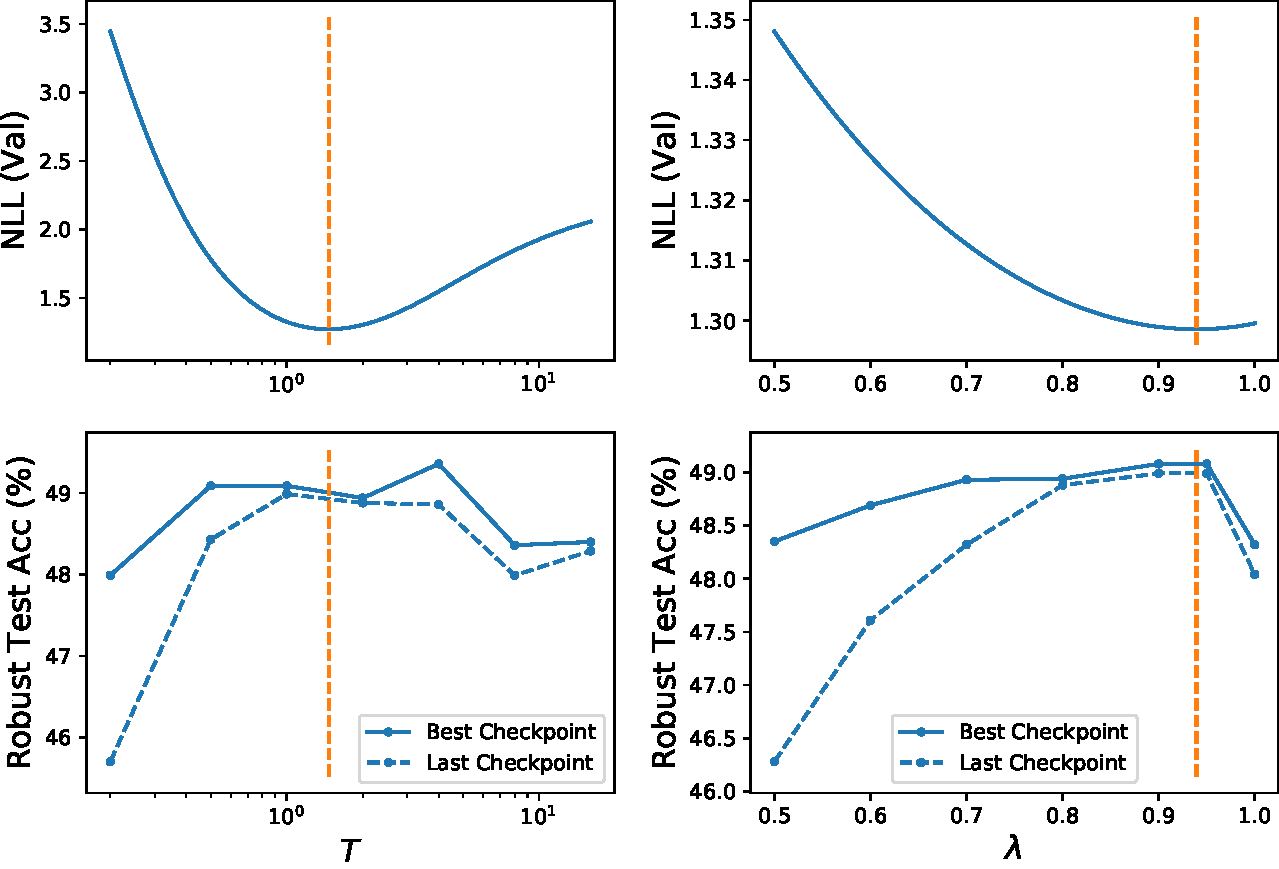
\includegraphics[width=1.0\linewidth]{figures/method-grid-search.pdf}
  \caption{(Upper) NLL loss obtained on the validation set for different $T$ and $\lambda$. (Bottom) Robust test accuracy at the best and last checkpoint by adversarial training with the rectified model probability with different $T$ and $\lambda$. $\lambda=0.8$ for grid search on $T$ (Left) and $T=2$ for grid search on $\lambda$ (Right). Orange dashed lines indicate $T$ and $\lambda$  determined by Equation~(\ref{eq:calibration}).}%
  \label{fig:method-grid-search}
  \vspace{-2cm}
% \end{figure}
\end{wrapfigure}




